\chapter{Results}

\section{Code Framework}
What?

\section{Drone Control}
\subsection{Rotation Script}
A python script was written to briefly take control of the drone and rotate while holding a constant position and altitude. The script used the Dronekit API provided by 3DR. The script was packed up with all necessary libraries and sent to the drone awaiting execution. When the command is given by a computer connected to the controller's WiFi network, the script runs, taking over control of the drone and rotating it. The API did not provide a way to set a constant rate of rotation, so instead a nonblocking call to rotate a certain amount was used in conjunction with timed sleeps to achieve a continuous rotation of 360 degrees. Attempts to map the script to a button on the controller were in vain. The 3DR developers guide notes a future API called "Smart Shots" that allows commands to be mapped to buttons on the controller, but it was not available at the time of this project.

\section{Localization}
\subsection{Mapping Script}
The script used to display the measured signal strengths was designed for post-proccesing use, taking in a text file of locations and their corresponding RSS values. The processing portion of the script is written in python. Equation \textbf{I NEED A REF} is used to calculate the raw distance to the signal. The Pythagorean Theorem is then used to eliminate the altitude component of the distance as can be seen in Figure \ref{fig:dist_pyth}. The latitude, longitude, and land-based distance are then formatted into a template string for each point at which a signal was detected.\par
\begin{figure}[ht]
\centering
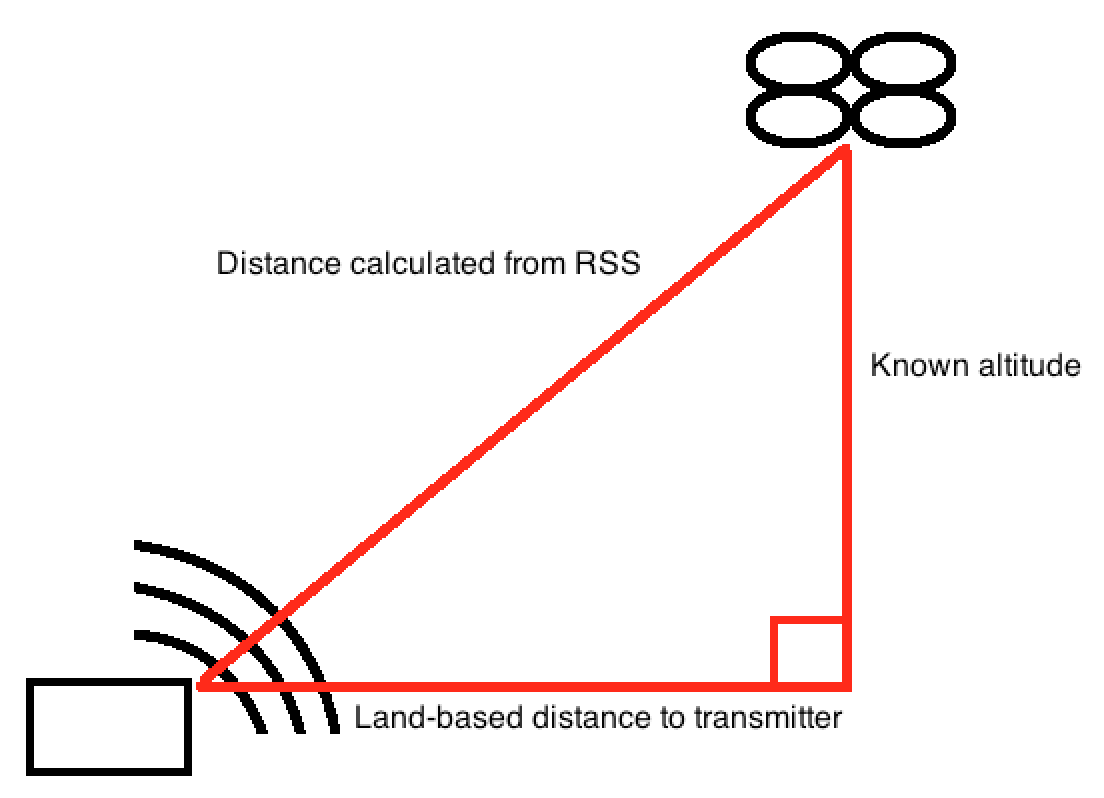
\includegraphics[width=0.70\textwidth]{img/distance_pythag_diagram.png}
\caption{Diagram showing right triangle used to calculate land-based distance from the calculated distance and a known altitude.}
\label{fig:map_localize}
\end{figure}
The formatted strings are inserted into a template html file, primarily composed of a javascript block that calls into the Google Maps API. Using the drawing tools in the API, rings are drawn on the map corresponding to the calculated distance. An example output screenshot of a generated map has been included in Figure \ref{fig:map_localize}. The actual output is a webpage with a Google Maps instance running in it, so the map is fully interactive, with the ability to zoom in and scroll around as well.
\begin{figure}[ht]
\centering
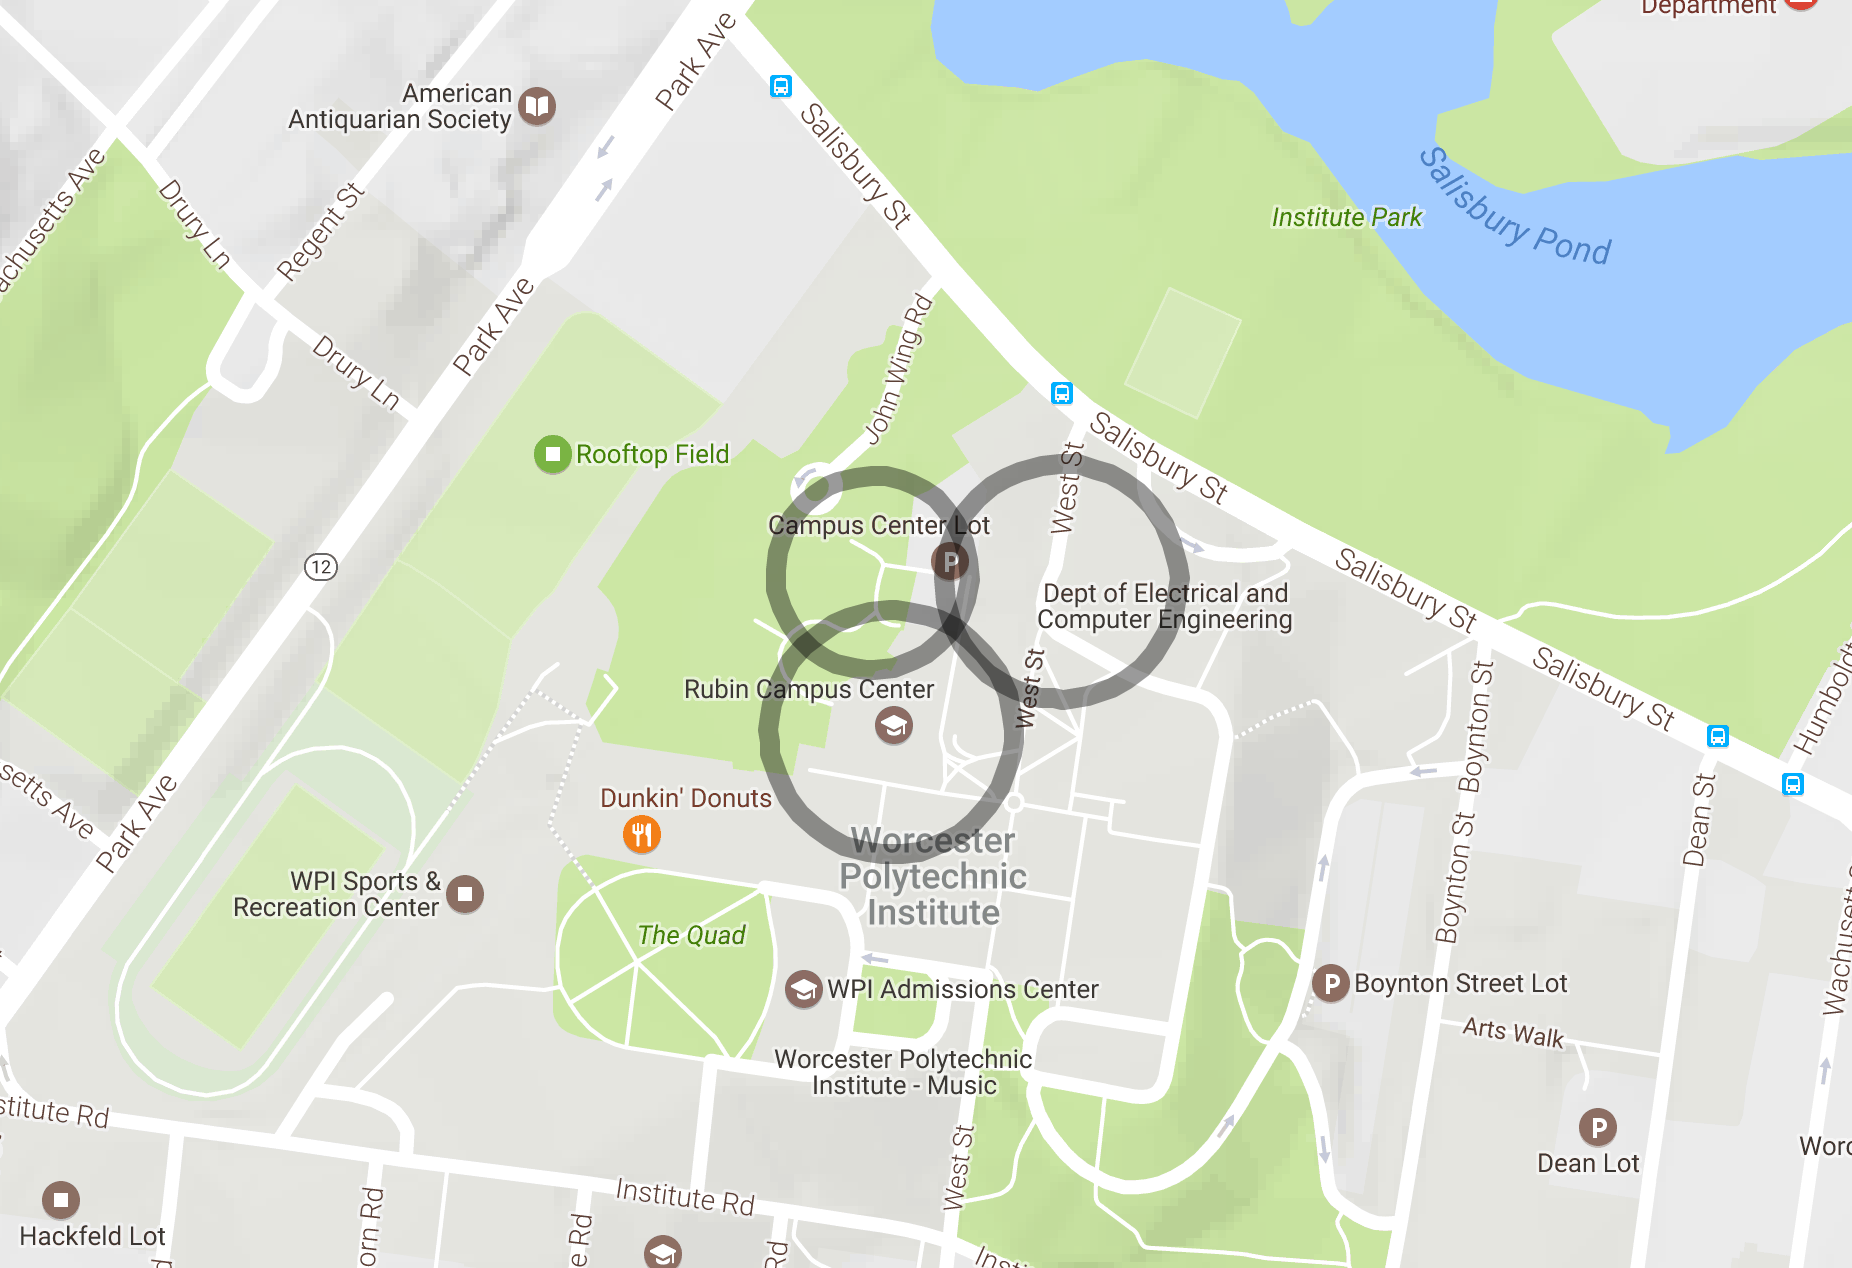
\includegraphics[width=0.70\textwidth]{img/localization_map_visualization.png}
\caption{Map-based localization example. The rings drawn are calculated from RSS values based on samples taken at the centers of each ring.}
\label{fig:map_localize}
\end{figure}